% This text is proprietary.
% It's a part of presentation made by myself.
% It may not used commercial.
% The noncommercial use such as private and study is free
% Sep. 2005 
% Author: Sascha Frank 
% University Freiburg 
% www.informatik.uni-freiburg.de/~frank/
%
% additional usepackage{beamerthemeshadow} is used
%  
%  \beamersetuncovermixins{\opaqueness<1>{25}}{\opaqueness<2->{15}}
%  with this the elements which were coming soon were only hinted
\documentclass{beamer}
\usepackage{beamerthemeshadow}
\usepackage{graphicx}
\usepackage{ifpdf}
\usepackage{url}
\usepackage{verbatim}
\usepackage{listings}
%\usepackage[demo]{graphicx}
\usepackage{caption}
\usepackage{subcaption}
\usepackage{cancel}
\usepackage[normalem]{ulem}
\usepackage{eurosym}
\begin{document}
\title{Parallel programming is \cancel{not} easy}
\author{Lukas van de Wiel}
\date{\today}

\frame{\titlepage}

\frame{\frametitle{Problem description}
A single thread computation... \\
\bigskip
\begin{tabular}{p{6cm}p{6cm}}
...does not fit in memory &  ...takes too long
\end{tabular}

\begin{figure}
\centering
\begin{subfigure}{.5\textwidth}
  \centering
  
\includegraphics[width=.7\linewidth]{images/elephant.jpg}
%  \caption{A subfigure}
  \label{fig:sub1}
\end{subfigure}%
\begin{subfigure}{.5\textwidth}
  \centering
  
\includegraphics[width=.7\linewidth]{images/hourglass.jpg}
%  \caption{A subfigure}
  \label{fig:sub2}
\end{subfigure}
%\caption{A figure with two subfigures}
\label{fig:test}
\end{figure}
}

\frame{\frametitle{Problem description}
A single thread computation... \\
\bigskip
\begin{tabular}{p{6cm}p{6cm}}
...does not fit in memory &  ...takes too long
\end{tabular}
\begin{center}

\includegraphics[width=.4\linewidth]{images/both.jpeg}
\end{center}
}


\frame{\frametitle{The dilemma}
Two ways to solve this: \\
\bigskip
\begin{center}
\begin{tabular}{p{3cm}p{3cm}}
spend time & spend money
\end{tabular}

\includegraphics[width=.6\linewidth]{images/scales.png}
\end{center}
}

\frame{\frametitle{What does money get you?}
CPU speed is limited, but memory is cheap (\euro 5.30 / GB):\\
\bigskip
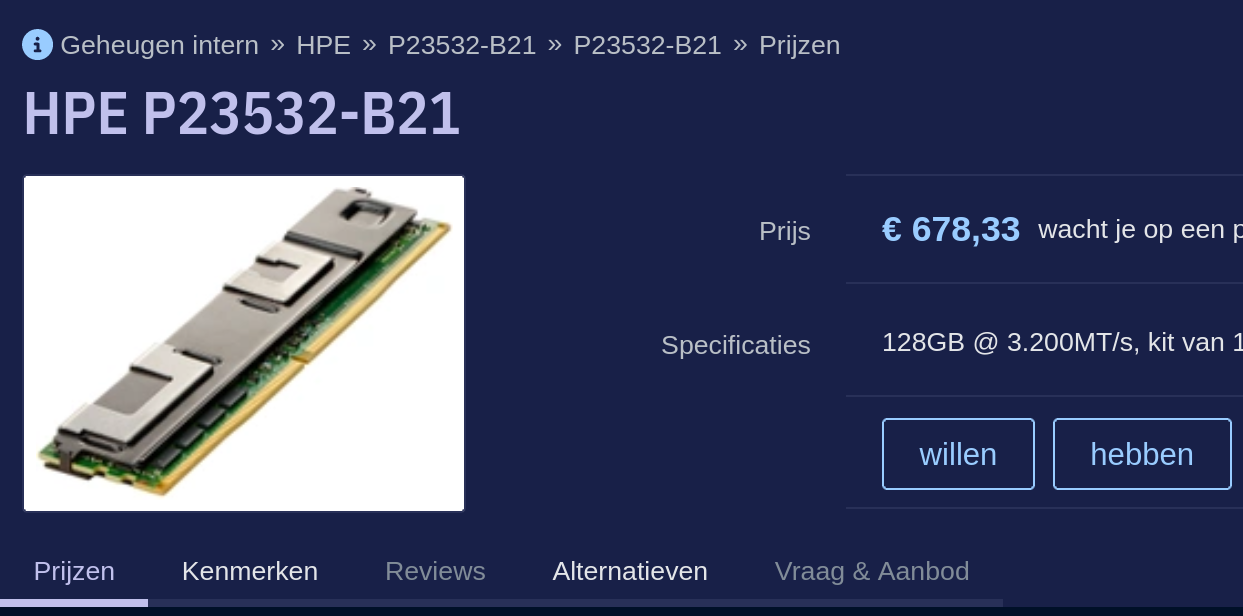
\includegraphics[width=\linewidth]{images/memorycrop.png}
}



\frame{\frametitle{What does time get you?}
Software optimization and parallellisation 
is all about time management. We face another choice between two options:\\
\bigskip

\begin{tabular}{p{5cm}p{5cm}}
Optimizing the code & Work on something else while the program runs
\end{tabular}

\begin{center}

\includegraphics[width=0.7\linewidth]{images/optimizeOrSomethingElse.png}
\end{center}

}



\frame{\frametitle{Is the software suitable for parallellisation?}
Can our algorithm be parallellised at all? Does the implementation have:
\begin{enumerate}
\item loops with independent operations?
\item independent processes?
\end{enumerate}
Good news!
\begin{enumerate}
\item Iterative algorithm
\end{enumerate}
Bad news!
}



\frame{\frametitle{Is the hardware suitable for parallellisation?}
When did we first get parallel hardware?
\begin{itemize}
\item first compute cluster: 1969 (ARPANET project)
\item first multicore processors: 2001 (IBM Power 4)
\end{itemize}

\bigskip
What is the state of parallel hardware today?
\begin{itemize}
\item highest CPU core count processor: 128  (AMD EPYC 9754)
\item highest GPU core count processor: 18.176  (NVIDIA RTX 6000 Ada)
\item biggest cluster: $\sim 2 \times 10^5$ CPU cores (Summit)
\end{itemize}
\bigskip
Even phones?
\begin{itemize}
\item Yes: 10 cores (Samsung Galaxy S24; Exynos 2400)
\end{itemize}
Single thread programming in 2024: Big Sad! 
\includegraphics[width=0.1\linewidth]{images/bigsad.png}
}



\frame{ \frametitle{How much do we need?}
\begin{center}
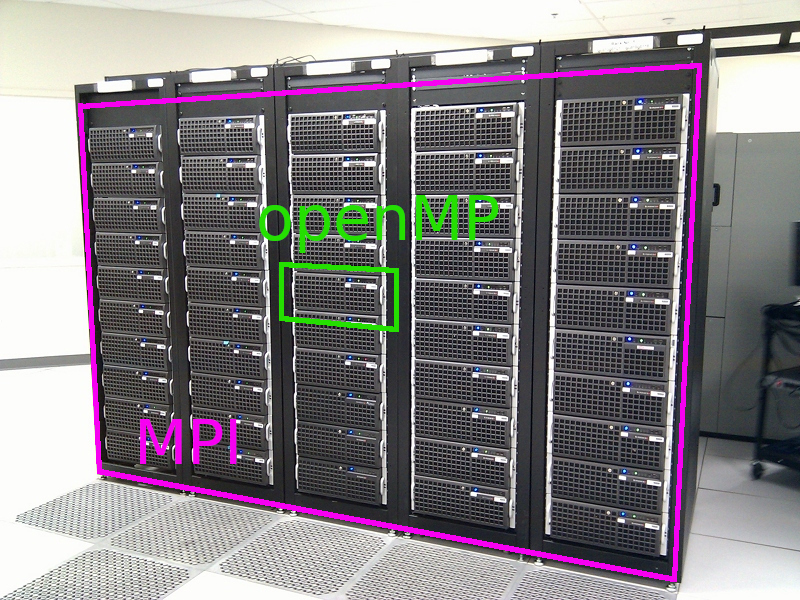
\includegraphics[width=0.85\linewidth]{images/realCluster.jpg}
\end{center}
10g cluster from Jefferson Lab
}

\frame{ \frametitle{openMP vs MPI}
\begin{center}
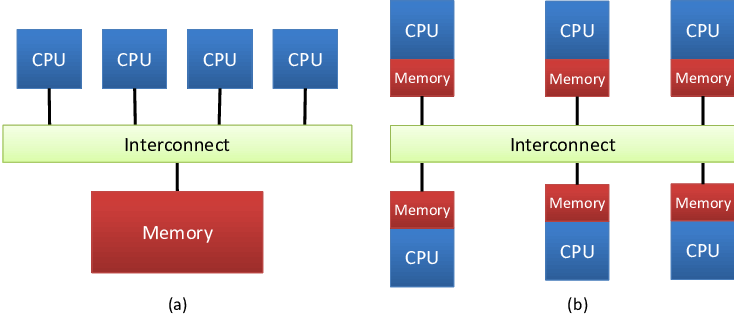
\includegraphics[width=\linewidth]{images/memoryTypes.png}
\end{center}
openMP (a) vs MPI (b). Source: Luciano Ost; \textit{Adaptation Strategies in Multiprocessors System on Chip}
}


\frame{ \frametitle{But how?}
\begin{center}
Let us look at some examples!
\end{center}
}



\defverbatim[colored]\lstNoOMP{
\begin{lstlisting}[language=Fortran,basicstyle=\ttfamily,keywordstyle=\color{red}]
integer          :: i
double precision :: a(800)

do i=1,800
  call doIndependentWork(a(i))
enddo
\end{lstlisting}
}


\frame{\frametitle{Without openMP. Serial. Slow:}
\bigskip
\lstNoOMP
}


\defverbatim[colored]\lstYesOMP{
\begin{lstlisting}[language=Fortran,basicstyle=\ttfamily,keywordstyle=\color{red}]
use omp_lib

integer          :: i
double precision :: a(800)

!$omp parallel do

do i=1,800
  call doIndependentWork(a(i))
enddo

!$omp end parallel do
\end{lstlisting}
}

\frame{\frametitle{With openMP. Parallel. Fast:}
\bigskip
\lstYesOMP
}

%\defverbatim[colored]\lstPythonNoOMP{
%\begin{lstlisting}[language=Python,basicstyle=\ttfamily,keywordstyle=\color{red}]
%same in Python, without openMP
%\end{lstlisting}
%}

\defverbatim[colored]\lstPyInv{
\begin{lstlisting}[language=Fortran,basicstyle=\ttfamily,keywordstyle=\color{red}]
import numpy

size = 10000

m  = numpy.random.random((size,size))
mi = numpy.linalg.inv(m)
\end{lstlisting}
}

\frame{\frametitle{Python}
\bigskip
Python suffers from GIL (Global Interpreter Lock): Only one thread can use the interpreter at any give time.\\
\bigskip
Python has no explicit openMP.\\
\bigskip
Parallel openMP-like functionality is used in C functions that are called through scipy/numpy/etc:\\
\bigskip

\lstPyInv

}



\defverbatim[colored]\lstMPI{
\begin{lstlisting}[language=Fortran,basicstyle=\ttfamily,keywordstyle=\color{red}]
use mpi

integer          :: i, iE, nProcs, myProcID, f
double precision :: a(800)

call mpi_init(iE)
call mpi_comm_rank(MPI_COMM_WORLD, myProcID, iE)

f = myProcID * 100 + 1

do i = f, f+99
  call doIndependentWork(a(i))
enddo

call mpi_finalize(iE)
\end{lstlisting}
}

\frame{ \frametitle{MPI, requires a bit more effort:}
\lstMPI
}


\defverbatim[colored]\lstdatacp{
\begin{lstlisting}[language=Fortran,basicstyle=\ttfamily,keywordstyle=\color{red}]
call mpi_bcast(...)
call mpi_scatter(...)
call mpi_gather(...)
call mpi_allgather(...)
\end{lstlisting}
}


\frame{ \frametitle{MPI, a more realistic example:}
But wait, we cheated! We ignored the `distributed memory' aspect of openMPI.
Each thread had all the input data (a) and only its own data computed, but no single thread has all the output:

\begin{center}
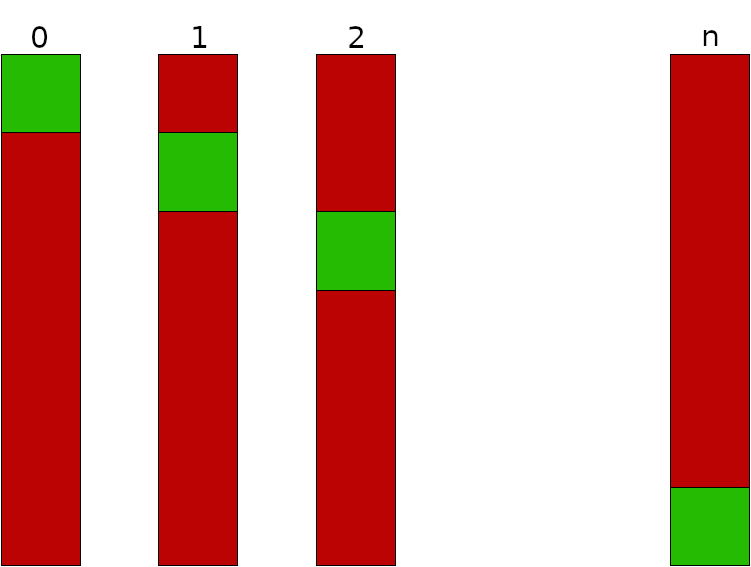
\includegraphics[width=0.7\linewidth]{images/myOwnData.png}
\end{center}

}




\frame{ \frametitle{MPI, a more realistic example:}

Real life situations are typically of the workflow:
\bigskip
\begin{enumerate}
\item Thread 0 reads input data from file.
\item Input data is distributed over all the threads.
\item All threads do their computations in parallel.
\item Results are copied back from each thread to thread 0.
\item Thread 0 writes output data to file.
\end{enumerate}

}

\frame{ \frametitle{So we need to copy data}
\begin{center}
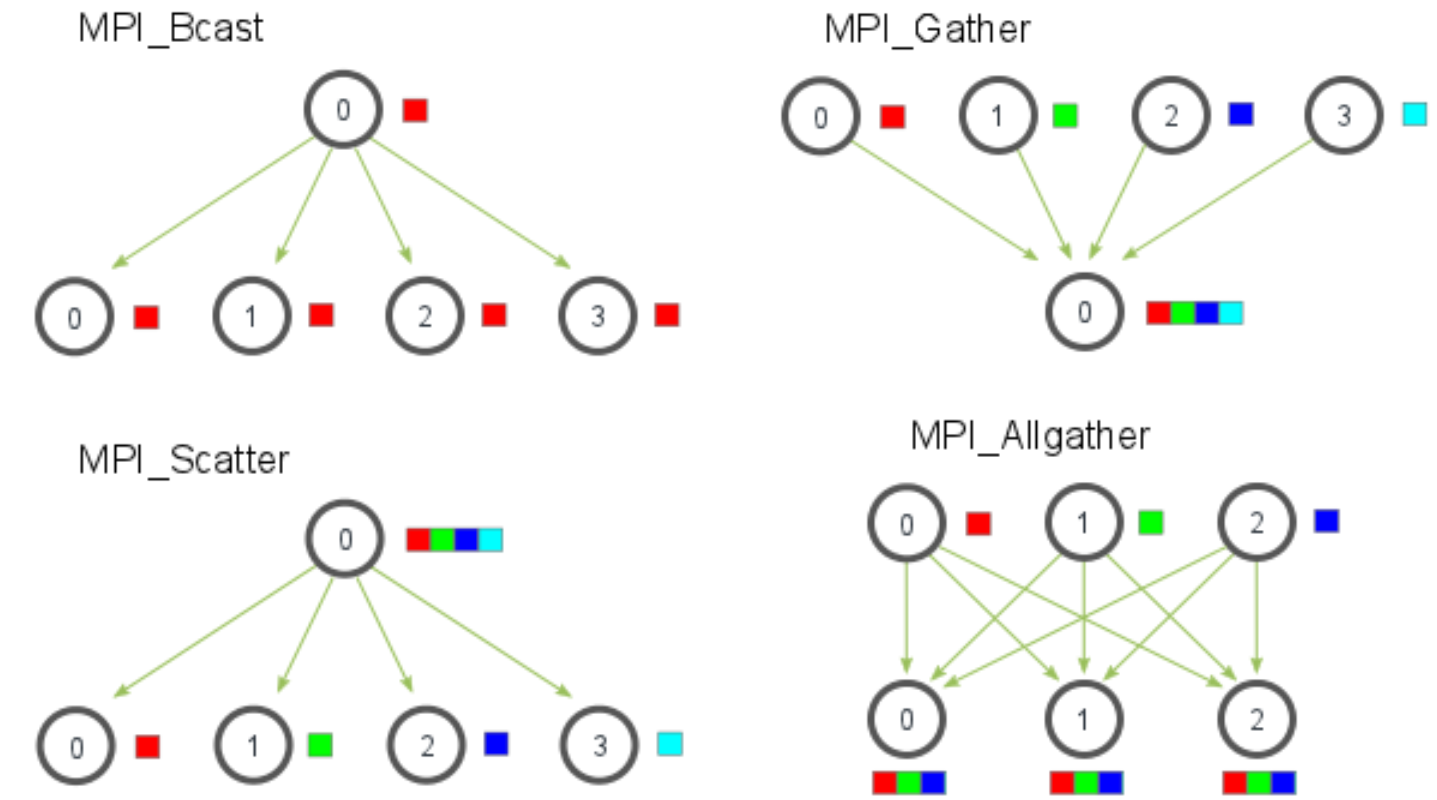
\includegraphics[width=\linewidth]{images/datacopy.png}
\end{center}
source: \url{https://mpitutorial.com/tutorials/mpi-scatter-gather-and-allgather/}
}



\defverbatim[colored]\lstPythonScatGath{
\begin{lstlisting}[language=Python,basicstyle=\ttfamily,keywordstyle=\color{red}]
from mpi4py import MPI
import numpy
globIn  = numpy.zeros(80)
globOut = numpy.zeros(80)
loc     = numpy.zeros(10)

rank = MPI.COMM_WORLD.Get_rank()

if rank == 0:
    globIn = numpy.loadtxt("inputData.txt")

MPI.COMM_WORLD.Scatter(globIn, loc, root=0)
loc = 10 * loc
MPI.COMM_WORLD.Gather(loc, globOut, root=0)

if rank == 0:
    numpy.savetxt("outData.txt", globOut)

\end{lstlisting}
}




\frame{ \frametitle{Python: the gentle version}
\lstPythonScatGath
}







\defverbatim[colored]\lstgather{
\begin{lstlisting}[language=Fortran,basicstyle=\ttfamily,keywordstyle=\color{red}]
MPI_Gather(
    void* send_data,
    int send_count,
    MPI_Datatype send_datatype,
    void* recv_data,
    int recv_count,
    MPI_Datatype recv_datatype,
    int root,
    MPI_Comm communicator,
    int error)
\end{lstlisting}
}

\defverbatim[colored]\lstscatter{
\begin{lstlisting}[language=Fortran,basicstyle=\ttfamily,keywordstyle=\color{red}]
MPI_Scatter(
    void* send_data,
    int send_count,
    MPI_Datatype send_datatype,
    void* recv_data,
    int recv_count,
    MPI_Datatype recv_datatype,
    int root,
    MPI_Comm communicator,
    int error)
\end{lstlisting}
}




\frame{ \frametitle{MPI, MPI\_Scatter}
\lstscatter
}

\frame{ \frametitle{MPI, MPI\_Gather}
\lstgather
}




\defverbatim[colored]\lstMPI{
\begin{lstlisting}[language=Fortran,basicstyle=\ttfamily,keywordstyle=\color{red}]
use mpi

double precision :: input(100)

call readInputData()
call mpi_init(iE)
call mpi_comm_size(MPI_COMM_WORLD, myProcID, iE)
call mpi_scatter(...)

f = myProcID * 100 + 1
do i = f, f+99
  call doIndependentWork(a(i))
enddo

call mpi_gather(...)
call writeOutputData()
call mpi_finalize(iE)
\end{lstlisting}
}


\defverbatim[colored]\lstImportMPIpy{
\begin{lstlisting}[language=Python,basicstyle=\ttfamily,keywordstyle=\color{red}]
import mpi4py
\end{lstlisting}
}

\frame{ \frametitle{MPI, Python}
\lstImportMPIpy

has a nice little extra!\\
\bigskip
send and receive datatype is no longer bound to MPI\_Datatypes.\\
\bigskip
Any object can be scattered and gathered!
}


\defverbatim[colored]\lstparrun{
\begin{lstlisting}[language=Python,basicstyle=\ttfamily,keywordstyle=\color{red}]
> mpirun -np 48 python3 myCoolCode.py
\end{lstlisting}
}



\frame{ \frametitle{MPI, Python, one little danger}

Remember the implicit parallellisation of the matrix inversion?\\

\bigskip

\lstparrun

\bigskip

Thread 0 thinks: I have 48 processors for my openMP processes!\\
Thread 1 thinks: I have 48 processors for my openMP processes!\\
Thread 2 thinks: I have 48 processors for my openMP processes!\\
Thread 3 thinks: I have 48 processors for my openMP processes!\\
Thread 4 thinks: I have 48 processors for my openMP processes!\\
...\\
}




\frame{ \frametitle{Scaling test}
\begin{center}

\includegraphics[width=0.7\linewidth]{images/scalingTestScales.png}
\end{center}
No scaling test? Not finished!
}


\frame{ \frametitle{Scaling test}
\begin{center}
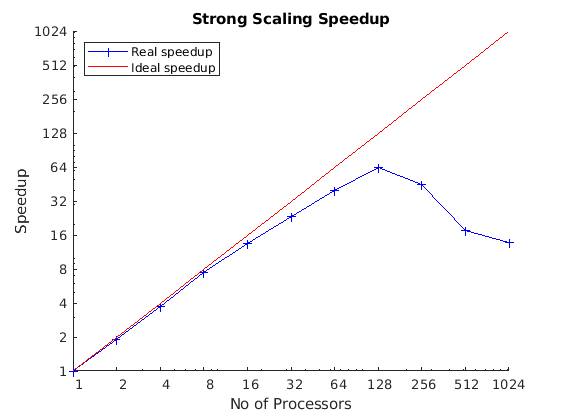
\includegraphics[width=0.8\linewidth]{images/Cg_speedup.png}
\end{center}

source: \url{https://hpc-wiki.info}
}















\frame{ \frametitle{Conclusion}
We have learned three things here:

\begin{enumerate}

\item Only go parallel when you have to. If you can get away with spending a small amount of 
money, or if you have other work to do while the software runs, that is the wiser option.

\item Take the easiest route of parallellisation. If OpenMP is enough, add a few tags and be done. If 
not, go full MPI.

\item Always test your scaling and find the optimal number of cores to run on.
\end{enumerate}

}


\frame{ \frametitle{The end}
Thread 0 says: Thank you for your time

\bigskip
Thread 1 says: Thank you for your attention

\bigskip
Thread 2 says: Find all material at: \url{github.com/LukasvdWiel/parProgIsEasy}

}



\end{document}
